\documentclass{article}
\usepackage[T1]{fontenc}
\usepackage{lmodern}
\usepackage{graphicx}
\usepackage{amsmath,amssymb}
\usepackage[a4paper,margin=2cm]{geometry}
\usepackage[absolute,overlay]{textpos}
\setlength{\TPHorizModule}{1mm}
\setlength{\TPVertModule}{1mm}
\usepackage[indonesian]{babel}
\usepackage{hyperref}
\setlength{\emergencystretch}{2em}
% unit: Halaman 8

\begin{document}

% === Halaman 8 (llm) ===

\begin{itemize}
    \item Enkripsi dan dekripsi Caesar Cipher dapat dilakukan secara matematis
    \item Misalkan setiap huruf alfabet dikodekan ke dalam integer dari 0 sampai 25 sebagai berikut:
\end{itemize}

\vspace{5mm}

\vspace{5mm}

maka, secara matematis Caesar Cipher dirumuskan sebagai:

\[ 
\text{Enkripsi: } c = E(p) = (p + 3) \pmod{26} \\
\text{Dekripsi: } p = D(c) = (c - 3) \pmod{26} 
\]

Ket: $p = \text{plainteks}; \quad c = \text{cipherteks}$

% deskripsi: Tabel pemetaan huruf alfabet (A-Z) ke nilai integer (0-25) untuk Caesar Cipher
% bbox normalisasi: [0.0680, 0.2900, 0.9530, 0.4230]
\begin{textblock*}{185.85mm}(14.28mm,86.13mm)
\noindent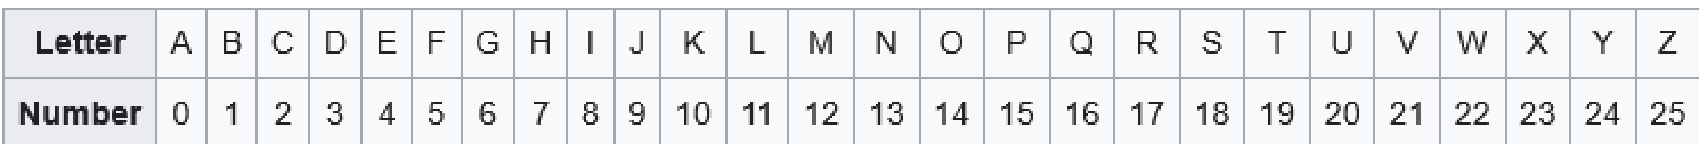
\includegraphics[width=185.85mm,height=39.50mm]{../../images/llm/page_008_img_01.png}%
\end{textblock*}

\end{document}
